% Options for packages loaded elsewhere
\PassOptionsToPackage{unicode}{hyperref}
\PassOptionsToPackage{hyphens}{url}
\PassOptionsToPackage{dvipsnames,svgnames,x11names}{xcolor}
%
\documentclass[
  12pt]{article}

\usepackage{amsmath,amssymb}
\usepackage{iftex}
\ifPDFTeX
  \usepackage[T1]{fontenc}
  \usepackage[utf8]{inputenc}
  \usepackage{textcomp} % provide euro and other symbols
\else % if luatex or xetex
  \usepackage{unicode-math}
  \defaultfontfeatures{Scale=MatchLowercase}
  \defaultfontfeatures[\rmfamily]{Ligatures=TeX,Scale=1}
\fi
\usepackage{lmodern}
\ifPDFTeX\else  
    % xetex/luatex font selection
\fi
% Use upquote if available, for straight quotes in verbatim environments
\IfFileExists{upquote.sty}{\usepackage{upquote}}{}
\IfFileExists{microtype.sty}{% use microtype if available
  \usepackage[]{microtype}
  \UseMicrotypeSet[protrusion]{basicmath} % disable protrusion for tt fonts
}{}
\makeatletter
\@ifundefined{KOMAClassName}{% if non-KOMA class
  \IfFileExists{parskip.sty}{%
    \usepackage{parskip}
  }{% else
    \setlength{\parindent}{0pt}
    \setlength{\parskip}{6pt plus 2pt minus 1pt}}
}{% if KOMA class
  \KOMAoptions{parskip=half}}
\makeatother
\usepackage{xcolor}
\setlength{\emergencystretch}{3em} % prevent overfull lines
\setcounter{secnumdepth}{5}
% Make \paragraph and \subparagraph free-standing
\makeatletter
\ifx\paragraph\undefined\else
  \let\oldparagraph\paragraph
  \renewcommand{\paragraph}{
    \@ifstar
      \xxxParagraphStar
      \xxxParagraphNoStar
  }
  \newcommand{\xxxParagraphStar}[1]{\oldparagraph*{#1}\mbox{}}
  \newcommand{\xxxParagraphNoStar}[1]{\oldparagraph{#1}\mbox{}}
\fi
\ifx\subparagraph\undefined\else
  \let\oldsubparagraph\subparagraph
  \renewcommand{\subparagraph}{
    \@ifstar
      \xxxSubParagraphStar
      \xxxSubParagraphNoStar
  }
  \newcommand{\xxxSubParagraphStar}[1]{\oldsubparagraph*{#1}\mbox{}}
  \newcommand{\xxxSubParagraphNoStar}[1]{\oldsubparagraph{#1}\mbox{}}
\fi
\makeatother


\providecommand{\tightlist}{%
  \setlength{\itemsep}{0pt}\setlength{\parskip}{0pt}}\usepackage{longtable,booktabs,array}
\usepackage{calc} % for calculating minipage widths
% Correct order of tables after \paragraph or \subparagraph
\usepackage{etoolbox}
\makeatletter
\patchcmd\longtable{\par}{\if@noskipsec\mbox{}\fi\par}{}{}
\makeatother
% Allow footnotes in longtable head/foot
\IfFileExists{footnotehyper.sty}{\usepackage{footnotehyper}}{\usepackage{footnote}}
\makesavenoteenv{longtable}
\usepackage{graphicx}
\makeatletter
\def\maxwidth{\ifdim\Gin@nat@width>\linewidth\linewidth\else\Gin@nat@width\fi}
\def\maxheight{\ifdim\Gin@nat@height>\textheight\textheight\else\Gin@nat@height\fi}
\makeatother
% Scale images if necessary, so that they will not overflow the page
% margins by default, and it is still possible to overwrite the defaults
% using explicit options in \includegraphics[width, height, ...]{}
\setkeys{Gin}{width=\maxwidth,height=\maxheight,keepaspectratio}
% Set default figure placement to htbp
\makeatletter
\def\fps@figure{htbp}
\makeatother

\addtolength{\oddsidemargin}{-.5in}%
\addtolength{\evensidemargin}{-1in}%
\addtolength{\textwidth}{1in}%
\addtolength{\textheight}{1.7in}%
\addtolength{\topmargin}{-1in}%
\makeatletter
\@ifpackageloaded{caption}{}{\usepackage{caption}}
\AtBeginDocument{%
\ifdefined\contentsname
  \renewcommand*\contentsname{Table of contents}
\else
  \newcommand\contentsname{Table of contents}
\fi
\ifdefined\listfigurename
  \renewcommand*\listfigurename{List of Figures}
\else
  \newcommand\listfigurename{List of Figures}
\fi
\ifdefined\listtablename
  \renewcommand*\listtablename{List of Tables}
\else
  \newcommand\listtablename{List of Tables}
\fi
\ifdefined\figurename
  \renewcommand*\figurename{Figure}
\else
  \newcommand\figurename{Figure}
\fi
\ifdefined\tablename
  \renewcommand*\tablename{Table}
\else
  \newcommand\tablename{Table}
\fi
}
\@ifpackageloaded{float}{}{\usepackage{float}}
\floatstyle{ruled}
\@ifundefined{c@chapter}{\newfloat{codelisting}{h}{lop}}{\newfloat{codelisting}{h}{lop}[chapter]}
\floatname{codelisting}{Listing}
\newcommand*\listoflistings{\listof{codelisting}{List of Listings}}
\makeatother
\makeatletter
\makeatother
\makeatletter
\@ifpackageloaded{caption}{}{\usepackage{caption}}
\@ifpackageloaded{subcaption}{}{\usepackage{subcaption}}
\makeatother
\ifLuaTeX
  \usepackage{selnolig}  % disable illegal ligatures
\fi
\usepackage[]{natbib}
\bibliographystyle{agsm}
\usepackage{bookmark}

\IfFileExists{xurl.sty}{\usepackage{xurl}}{} % add URL line breaks if available
\urlstyle{same} % disable monospaced font for URLs
\hypersetup{
  pdftitle={Zoning: A Barrier or Solution to Truck Parking Infrastructure Shortages?},
  pdfauthor={William Co},
  colorlinks=true,
  linkcolor={blue},
  filecolor={Maroon},
  citecolor={Blue},
  urlcolor={Blue},
  pdfcreator={LaTeX via pandoc}}


\begin{document}


\def\spacingset#1{\renewcommand{\baselinestretch}%
{#1}\small\normalsize} \spacingset{1}


%%%%%%%%%%%%%%%%%%%%%%%%%%%%%%%%%%%%%%%%%%%%%%%%%%%%%%%%%%%%%%%%%%%%%%%%%%%%%%

\date{February 3, 2025}
\title{\bf Zoning: A Barrier or Solution to Truck Parking Infrastructure
Shortages?}
\author{
William Co\thanks{true}\\
Department of Economics, University of British Columbia\\
}
\maketitle

\bigskip
\bigskip
\begin{abstract}
This study explores the impact of local zoning regulations on the
growing shortage of truck parking in the United States. We utilize
traffic accident data as a proxy for truck parking demand to examine how
zoning restrictions affect parking capacity. Employing an event study
design, we categorize zoning regimes into Traditional, Exclusion,
Reform, and Wild Wild Texas. Additionally, we implement a
difference-in-differences approach to compare high-restrictive and
low-restrictive areas.
\end{abstract}


\newpage
\spacingset{1.9} % DON'T change the spacing!

\section{Agenda}\label{agenda}

\begin{enumerate}
\def\labelenumi{\arabic{enumi}.}
\item
  Quantifying Truck Parking Shortage.~
\item
  Do local economies respond to the need for truck parking or is it
  hindered?
\item
  Does land regulation limit truck parking creation?
\end{enumerate}

\section{Research Question}\label{research-question}

What is the effect of truck parking accidents on truck stop creation?

\section{Motivation}\label{motivation}

\subsection{Magnitude}\label{magnitude}

The ongoing truck parking crisis in the United States presents
significant challenges to truck drivers, the freight transportation
industry, and overall public safety. According to the American
Transportation Research Institute (ATRI), truck drivers lose an average
of 56 minutes of driving time per day searching for safe and legal
parking facilities. This inefficiency results in an annual economic loss
of approximately \$5,600 per driver. Given that there are 3.874 million
truck drivers in North America, as reported by the U.S. Bureau of Labor
Statistics and Statistics Canada, this translates to an industry-wide
financial loss of \$21.69 billion annually, exacerbating economic strain
on a sector crucial to national and international commerce.

\subsection{Truck Parking as a Primary Industry
Concern}\label{truck-parking-as-a-primary-industry-concern}

The scarcity of truck parking has consistently ranked as the most
pressing issue within the trucking industry, as identified in ATRI's
annual industry reports. The problem is particularly severe in
metropolitan areas, where the demand for freight transportation is high,
yet local regulations and public opposition hinder the development of
additional truck parking facilities. The current parking capacity is
grossly inadequate, with only one available parking space for every 11
semi-trucks on the road, leading to a nationwide shortfall exceeding
40,000 spaces. Consequently, many truck drivers are compelled to park in
unsafe or unauthorized locations, thereby increasing their exposure to
accidents, cargo theft, and regulatory violations.

The Federal Motor Carrier Safety Administration (FMCSA) mandates that
truck drivers adhere to Hours-of-Service (HOS) regulations, which
require a 10-hour rest period after 11 consecutive hours of driving.
However, the lack of available parking forces drivers into suboptimal
decisions, including continuing to drive while fatigued, parking
illegally, or violating HOS regulations. According to ATRI,
approximately 70\% of drivers report difficulty in securing safe and
legal parking, while over 90\% indicate that this challenge negatively
impacts their quality of life. The Federal Highway Administration
further corroborates these findings, reporting that 98\% of truck
drivers experience difficulties locating secure rest areas, which
contributes to stress, fatigue, and long-term health issues among
drivers.

Despite the widespread recognition of this issue, efforts to mitigate
the crisis have been hindered by public opposition to the construction
of new truck parking facilities. Surveys indicate that while the
majority of respondents acknowledge the necessity of additional truck
parking, 80\% oppose the construction of such facilities within a
three-mile radius of their residences, with 5\% rejecting the notion
outright. This incongruity between awareness and action complicates
policymaking and infrastructure development efforts aimed at resolving
the crisis.

\subsection{Economic and Infrastructure
Implications}\label{economic-and-infrastructure-implications}

The economic ramifications of the truck parking crisis extend beyond
individual truck drivers to the broader freight transportation industry
and national economy. In 2022, the trucking industry transported \$948
billion in freight, with employment in the sector expanding by 8\%.
However, the development of truck parking infrastructure has not kept
pace with industry growth, exacerbating the parking shortage.
Additionally, unauthorized parking on highways and rest areas
contributes to increased congestion and accelerates infrastructure
deterioration, thereby imposing substantial maintenance costs on state
and federal governments.

The absence of sufficient legal parking compels truck drivers to stop in
hazardous locations, including highway shoulders, entrance and exit
ramps, and unauthorized rest areas. A Federal Highway Administration
study indicates that 43.8\% of trucks are parked illegally overnight.
Such practices not only jeopardize driver safety but also endanger other
motorists by reducing roadway visibility and increasing the probability
of collisions.

\subsection{Health and Safety
Concerns}\label{health-and-safety-concerns}

The shortage of truck parking also has significant implications for the
physical and mental well-being of truck drivers. Extended searches for
parking increase stress levels, contribute to sleep deprivation, and
elevate the risk of fatigue-related accidents. Some trucking companies
utilize GPS-based tracking systems that automatically shut down trucks
when drivers reach their HOS limits, potentially leaving them stranded
in unsafe locations. If a designated parking spot cannot be found in
time, some trucks may shut down on the side of the highway, exposing
drivers to serious risks.

Moreover, inadequate parking infrastructure heightens the risk of cargo
theft. According to the Supply Chain Intelligence Center, 75\% of cargo
theft incidents occur in unsecured parking locations, resulting in
millions of dollars in losses for the trucking industry. The case of
Jason Rivenburg underscores the grave dangers posed by insufficient
secure parking. In 2009, Rivenburg, a truck driver, was murdered during
a robbery while parked at an abandoned gas station due to a lack of safe
overnight parking. His death led to the enactment of Jason's Law (2012),
a federal initiative aimed at increasing funding for truck parking
facilities to enhance driver safety.

\subsection{Zoning}\label{zoning}

The United States hosts 90,056 local governments, each imposing unique
zoning restrictions that shape land use. Cities with bustling economies
require robust transportation logistics, including an adequate trucking
supply chain, to support economic growth. However, these thriving urban
centers often enforce strict zoning regulations that aim to protect land
values, promote housing development, and maintain order. Unfortunately,
these regulations frequently hinder the development of truck stops,
which are vital for the trucking industry to meet the demands of the
growing economy.

Zoning regulations have often been criticized for their inefficiencies
and unintended consequences. These inefficiencies are particularly
evident in areas such as low-cost housing, racial segregation,
productive land use, and commercial real estate, including office spaces
and housing price volatility
\citet{glaeserImpactBuildingRestrictions2003}.;
\citet{galeReviewColorLaw2019}; \citet{PDFTriumphCity2024} The
inefficiencies of zoning regulations in these other sectors are mirrored
in the truck parking crisis.

Despite the significant implications, there is limited empirical
research quantifying the relationship between truck parking creation and
the regulatory environment influencing its availability. Zoning
regulations, in particular, often play a more decisive role in truck
parking accessibility than geographic or transportation network factors
\citep{shertzerZoningEconomicGeography2018}. This study seeks to bridge
this gap by leveraging traffic accident data as a proxy for truck
parking demand and analyzing how zoning regulations impact truck parking
creation.

Addressing the growing need for truck stops in cities with strict zoning
regulations is essential to ensuring the safety of truckers and the
public while supporting the supply chain vital to these economies.

\section{Remark: Scale of Truck Parking Challenges
vs.~Homelessness}\label{remark-scale-of-truck-parking-challenges-vs.-homelessness}

While homelessness is a critical and deeply concerning issue in North
America, the shortage of truck parking presents a significantly larger
challenge in terms of sheer numbers. According to data from the U.S.
Bureau of Labor Statistics and Statistics Canada, there are
approximately 3.5 million truck drivers operating in the U.S. and
Canada. Studies indicate that a substantial percentage of these drivers
face difficulties finding safe and adequate parking.

A conservative estimate from the Federal Highway Administration (FHWA)
suggests that 43.8\% of truck drivers experience parking challenges,
translating to roughly 1.53 million affected drivers. However, other
estimates are even higher---research from the American Transportation
Research Institute (ATRI) has found the number to be closer to 70\%,
while the U.S. Department of Transportation (USDOT) has reported figures
as high as 98\%.

For comparison, the total homeless population in North
America---including the U.S. (\textasciitilde580,000), Canada
(\textasciitilde235,000), and Mexico (\textasciitilde50,000)---amounts
to approximately 865,000 individuals. This means that even under the
conservative FHWA estimate, the truck parking crisis affects nearly
twice as many people as the entire homeless population of North America.

While both issues are important, this analysis shows the scale of the
truck parking crisis, making it an even larger problem---if not at least
as significant---as the homelessness crisis affecting all of North
America.

\section{Conceptual Framework}\label{conceptual-framework}

Is zoning regulation welfare-enhancing? This paper examines this
question through the lens of trucking accidents. Areas with a high
frequency of trucking accidents can serve as evidence for the need to
relax zoning regulations, particularly those contributing to an
under-supply of truck parking. By analyzing these areas, we can compare
regions with strict zoning regulations to those with more lenient zoning
practices to identify discrepancies in truck parking availability.

Although several models exist to investigate whether zoning regulations
optimize welfare, none of these studies explicitly consider truck
parking as a variable. This research aims to fill that gap by
highlighting the relationship between zoning regulations, truck parking
availability, and their impact on trucking accidents, offering new
insights into the welfare implications of zoning policies.

Specifically, this research aims to test two hypotheses:

\begin{enumerate}
\def\labelenumi{\arabic{enumi}.}
\item
  If restrictive local zoning laws drive truck parking shortages,
  regions with high truck parking-related accidents should exhibit
  minimal correlation with increased truck stop capacity.
\item
  Parking accidents involving trucks can serve as a quantitative proxy
  for truck stop demand, enabling the evaluation of truck stop shortages
  across regions.
\end{enumerate}

this study employs an event study design, categorizing zoning regimes
into four types---Traditional, Exclusion, Reform, and Wild Wild
Texas---based on \citep{puentesTraditionalReformedReview2006} (See
\phantomsection\label{sec:appendix-b}\hyperref[sec-b.-map-of-zoning-categories]{Appendi}\hyperref[sec:appendix-b]{x
B}) . We hypothesize that restrictive zoning regimes (Traditional and
Exclusion) are less responsive to truck parking demand compared to
flexible regimes (Reform and Wild Wild Texas), resulting in lower truck
parking capacity despite evident needs.

Additionally, this study will employ a difference-in-differences design
to compare high-restrictive zoning areas with low-restrictive zoning
areas. By controlling for the four zoning categories---Traditional,
Exclusion, Reform, and Wild Wild Texas---we analyze the effects of a
major trucking accident as the event of interest. This approach will
allow us to assess how zoning restrictiveness influences truck parking
capacity and whether high-restrictive regimes exacerbate the challenges
associated with truck parking shortages in the aftermath of such
incidents.

\section{Related Literature}\label{related-literature}

Existing studies on zoning provide valuable context but are limited in
scope. Research often focuses on single areas (Chicago, Eastern
Massachusetts) and are often focused on aspects unrelated to truck
zoning regulation
\citep{shertzerRaceEthnicityDiscriminatory2016, glaeserCausesConsequencesLand2009}
or are scoped in international contexts such as Brazil
\citep{anagolEstimatingEconomicValue2021}. Furthermore, most literature
emphasizes US residential zoning
\citep{lensStrictLandUse2016, huangResidentialLandUse2012}or office
space \citep{cheshireOfficeSpaceSupply2008}, leaving industrial zoning
and its implications for truck parking largely unexplored. All of these
papers demonstrate that zoning reforms are binding and limit overall
population welfare in favor of benefiting a select few.

Initially designed to balance public welfare and economic development,
zoning regulations have evolved, sometimes adapting to market forces or
catering to local stakeholder interests, such as middle-class homeowners
\citep{fischelEconomicHistoryZoning2024}. While zoning has the potential
to enhance economic productivity, it can also introduce inefficiencies,
particularly in industrial applications
\citep{mcdonaldPDFEconomicsZoning2012}. Fragmented zoning governance
often discourages communities from accommodating truck parking, despite
its regional benefits, due to localized decision-making dynamics.
Furthermore, it is unclear whether the current state of land regulation
optimizes welfare. Some estimates say misallocation through zoning
welfare cost the economy up to 13.6 percent of gross domestic product
\citep{osmanRestrictiveLandUse2020}. This paper aims to address this gap
within the context of truck parking shortages these challenges,.

This research contributes to the broader discourse on zoning's economic
impact, extending the analysis to the critical issue of truck parking
infrastructure. By examining the interplay between zoning
classifications, parking-related accidents, and truck stop capacity,
this study offers insights for policymakers aiming to mitigate the
externalize of inadequate truck parking through thoughtful zoning
reforms.

\section{Contribution}\label{contribution}

This methodology has not been explored before primarily due to data
limitations and the recent emergence of the problem. Supply chain
strains and zoning restrictiveness are relatively recent phenomena. For
instance, Jason's Law, arguably the most significant legislation
addressing truck parking issues, only came into effect in 2012. The rise
of e-commerce, coupled with aging populations and increasing NIMBY-ism,
has exacerbated supply chain challenges in recent years.

Furthermore, the data set used in this study was compiled from digitized
versions of trucking directories, which traditionally do not publish
their data electronically. This data has only recently become available
thanks to the efforts of Prof.~Ron Yang's research group, who worked to
digitize and organize these records. This unique data set and the
recency of the issue make our study a novel empirical contribution to
the field.

\section{Data}\label{data}

Our data is (1990-Present) FMCA (Federal Motor Carrier Safety
Administration) Crash file from USDOT (Department of Transportation)
(\phantomsection\label{sec:appendix-a}\hyperref[sec-a.-visualization-of-dataset.-]{Appendix
A}). We can see type of vehicle (ex. trucks), nature of the crash (ex.
Crashed involving a ``parked'' vehicle), fatalities, injuries, number of
vehicles involved, etc. We will aslo use WLIURA (zoning restriction
index) dataset by \citet{gyourkoNewMeasureLocal2008} and zoning
classifications used by \citet{puentesTraditionalReformedReview2006} .
There are other papers like \citet{liangSafetyInspectionsImprove2021},
which use similar data sets.

\section{\texorpdfstring{\textbf{Strategy}}{Strategy}}\label{strategy}

With no truck parking available trucks illegally park causing observed
accidents such that plcaes increase truck parking availability, through
increase truck stop creation.

No Truck Parking → Trucks will illegally park → \textbf{Accidents Occur}
(observed)→Truck Parking Demand increases → \textbf{Truck Parking
Capacity Increase} (observed)

\subsection{Event Study Model}\label{event-study-model}

The equation to estimate the effect of the Truck Parking Accident (TPA)
on the creation of truck stops is specified as follows:

\[
\Delta \text{NumTruckStop}_{tj} = \sum_{i=-n}^{n} \beta_{ij} \text{Accident}_{ij}\cdot \text{Severity}_{ij} + \gamma_{tj} X_{tj} + \epsilon_{tj}
\]

Where:

\begin{itemize}
\item
  \(\Delta\text{NumTruckStop}_{tj}\) is the change in truck stop
  capacity in year \(t\) for category \(j\).
\item
  \(\beta_{ij}\) are the coefficients for the event dummies
  (\(\text{TPA}_{i,j}\)), where \(i\) represents the relative time unit
  to the Truck Parking Accident at \(i = 0\).
\item
  \(\text{Accident}_{i,j}\) is the event dummy indicating the presence
  of a Truck Parking Accident in relative year \(i\) for category \(j\).
  Specifically, when \(i = 0\), this corresponds to the year in which
  the Truck Parking Accident occurs.
\item
  \(\text{Severity}_{ij}\) takes the form of fatalities associated with
  the accident at time \(i\) and category \(j\).
\item
  \(\gamma\) represents the coefficients for the control variables
  (\(X_{tj}\)).
\item
  \(X_{tj}\) are the control variables in year \(t\) for category \(j\).
\item
  \(\epsilon_{tj}\) is the error term for year \(t\) and category \(j\).
\item
  \(j\) indicates a specific category used to isolate subsets of the
  data, discussed below.
\end{itemize}

To analyze the impact of the Truck Parking Accident across different
zoning categories, I will estimate to each corresponding category:

\begin{itemize}
\item
  Traditional: This category evaluates the effects in conventional
  settings with typical zoning regulations.
\item
  Exclusion: This category examines the impacts in areas where truck
  stops are limited or restricted by zoning laws.
\item
  Reform: This category focuses on regions undergoing policy or
  structural reforms related to truck parking.
\item
  Wild Wild Texas: This category investigates the unique circumstances
  and effects in Texas, a state known for its lack of zoning regulation.
\end{itemize}

\section{Adjusted Model for Truck Parking
Analysis}\label{adjusted-model-for-truck-parking-analysis}

Our dataset cannot accommodate the initial model because we only observe
changes in truck parking during the years 2007, 2008, 2015, and 2016. To
address this limitation, we adjust the model as follows:

\[
\Delta \text{NumTruckStop}_{j,t=2006-2016} = \sum_{i=-2}^{0} \beta_{j,t+i} \text{Accident}_{j,t+i}\cdot \text{Severity}_{j,t+i} + \gamma_{tj} X_{tj} + \epsilon_{tj}
\]

\subsection{Model Explanation}\label{model-explanation}

\begin{itemize}
\tightlist
\item
  \$ \text{TPA}\_\{t-i\} \$: A lagged dummy variable indicating a severe
  truck parking accident.
\item
  Severity is our measure of severity of the accident which can take the
  form of `VEHICLES\_IN\_ACCIDENT', `INJURIES' and fatalities
\item
  \$ i \$: Represents time units relative to the 2006-2016 period.
\item
  \$ X\_t \$: Includes control variables.
\item
  \$ \epsilon\_t \$: Error term.
\end{itemize}

This adjustment allows us to analyze the effects of severe truck parking
accidents within the available time frame.

\subsection{Difference-in-Differences (DiD)
Model}\label{difference-in-differences-did-model}

I will employ a Difference-in-Differences (DiD) design using the WLRUI
index data to compare locations with a high restriction index against
those with a low restriction index, while controlling for different
zoning categories. The model is specified as follows:

\[
Y_{tj} = \sum_{t=-n}^{n} \theta_{tj} HR_{tj} + \sum_{t=-n}^{n} \phi_{tj} Post_{tj} + \sum_{t=-n}^{n} \psi_{tj} (HR_{tj} \times Post_{tj}) + \gamma_{tj} X_{tj} + \epsilon_{tj}
\]

Where:

\begin{itemize}
\tightlist
\item
  \(Y_{tj}\) denotes the change in truck parking capacity for category
  \(j\) at time \(t\).
\item
  \(HR_{tj}\) indicates the high restriction index for category \(j\) at
  time \(t\).
\item
  \(Post_{tj}\) represents the indicator for the post-TPA period for
  category \(j\) at time \(t\).
\item
  \(HR_{tj} \times Post_{tj}\) is the interaction term that captures the
  treatment effect of being in a high restriction area following the
  truck parking accident.
\item
  \(\theta_{tj}\) represents unique coefficients for the high
  restriction index across both time periods \(t\) and categories \(j\).
\item
  \(\phi_{tj}\) indicates unique coefficients for the post-TPA period
  across both time periods \(t\) and categories \(j\).
\item
  \(\psi_{tj}\) reflects unique coefficients for the interaction term
  across both time periods \(t\) and categories \(j\).
\item
  \(\gamma_{tj}\) denotes unique coefficients for the control variables
  across both time periods \(t\) and categories \(j\).
\item
  \(X_{tj}\) is a vector of control variables for category \(j\) at time
  \(t\).
\item
  \(\epsilon_{tj}\) is the error term.
\end{itemize}

\section{\texorpdfstring{\textbf{Limitations}}{Limitations}}\label{limitations}

Data only indicates any accidents involving any parked vehicle. The
parked vehicle in question need not be a truck. The parked vehicle may
also be a legally parked truck.~ Im only targeting once aspect of
trucking accidents that are due to lack of truck parking. There are
tother causes of lack of truck parking like driin gin bad conditions. We
dont know wh is at fault. A innocent truck driver could eb invovled in
the accident. A sedan could be drunk on hit a pillagely parked truck

time variation. it may be the case that places change but we are only
observing 2006 and not 2024.

\section{\texorpdfstring{\textbf{Robustness}}{Robustness}}\label{robustness}

Buses, as a category of large vehicles, may be comparable to trucks in
some contexts, potentially introducing noise into our results. To ensure
robustness, we propose conducting the study both with and without buses
included in the dataset.

Accidents can be categorized as fatalities, injuries, or vehicles
involved, each requiring its own specific dependent variable response.
To address this, we will run our analysis separately for each category,
treating them as controls.

Concerns may arise regarding the time variation of zoning
classifications. However, this concern can be safely excluded, as zoning
regimes or classifications tend to remain relatively stable across
municipalities \citep{mclaughlinLandUseRegulation2012}.

\section{\texorpdfstring{\textbf{Improvements}}{Improvements}}\label{improvements}

There are other data sets found in \citep{NHTSAFileDownloads} or
\citep{FatalityAnalysisReporting} ; . That contain data that could
potentially be more relevant that addresses any limitations in our
design.

Insurance claims dataset are also another dataset worth looking into

\href{https://data.transportation.gov/Trucking-and-Motorcoaches/Motor-Carrier-Crash-Data-/b8e5-isfj/about_data}{Motor
Carrier Crash Data - \textbar{} Department of Transportation - Data
Portal}

\citet{liangSafetyInspectionsImprove2021} points out that state level
Texas DOT, has dataset that contain a more detailed infromation on the
trucking accident. Such as the source, of the accident why it happened
who is at fault and so forth. It has data on the exact cause of the
accident. Wheereas FMCA, data only contains general information on the
cirucsmtances of teh accident.

\section{Remarks}\label{remarks}

Most research on zoning restrictiveness focuses on housing, yet there is
no reason to believe that a housing restrictiveness index cannot be
adapted for studying industrial zoning restrictiveness.

Ideas to explore would include investigating trade offs between fatigue
driving and illegal parking. another avenue would be to investigate
overall accidents as well, isolating fatigued driving.

\section{\texorpdfstring{\textbf{Appendix}}{Appendix}}\label{appendix}

\subsection{\texorpdfstring{\textbf{A. Visualization of
dataset.}}{A. Visualization of dataset.}}\label{sec-a.-visualization-of-dataset.-}

(Present Truck stop parking observatios also available
\href{https://data-usdot.opendata.arcgis.com/datasets/usdot::truck-stop-parking/about}{Truck
Stop Parking \textbar{} Geospatial at the Bureau of Transportation
Statistics})

{[} \citet{coWilliamClintCResearchProposalTrucks2024}{]}

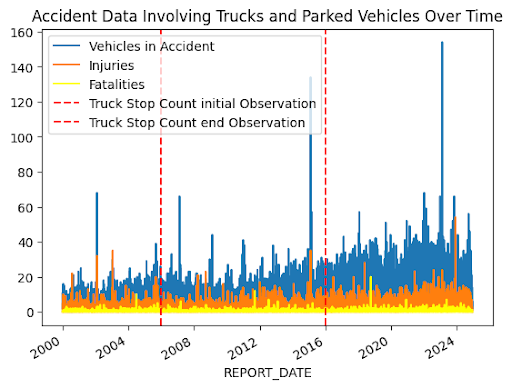
\includegraphics{images/unnamed.png}

\subsection{B. Map of Zoning
Categories}\label{sec-b.-map-of-zoning-categories}

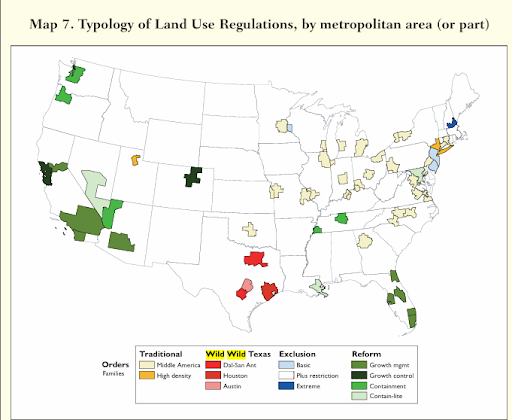
\includegraphics{images/unnamed (1).png}


  \bibliography{bibliography.bib}


\end{document}
